\todo{Update with numbers from Google Cloud}
\todo{Fix figures}

Our evaluation seeks to answer six questions:
%
\begin{enumerate}[nosep]
 %
 \item How much developer effort and application modification does \sys require? (\S\ref{s:eval-effort})
%
\item How expensive are common application operations, as well as
  \xxing, revealing, and operations over \xxed data with \sys? (\S\ref{s:eval-ops})
 %

\item What overheads does \sys impose, and where do they come from?
    (\S\ref{s:eval-overheads})

\item 
    How does the effort required to implement \sys's
    functionality in a related system (Qapla~\cite{qapla}),
    and its performance, compare with using \sys?
    (\S\ref{s:eval-qapla})

\item 
    What is the performance impact of composing \sys's guarantees
    with those of encrypted databases?
        (\S\ref{s:eval-cryptdb})

\item 
    Which categories of application updates and schema migrations can \sys
        support? (\S\ref{s:eval-updates})
%
\end{enumerate}

We compare Edna to three alternative settings:
\one{} a manual version
of each \xxing transformation that directly modifies the database
(\eg via SQL queries that remove data), which
lacks support for revealing and does not support
composition of multiple transformations;
\two{} an implementation of disguising and revealing in Qapla~\cite{qapla}
using Qapla’s query rewriting and access control policies; and \three{} an integration of Edna with CryptDB~\cite{cryptdb}, an encrypted database.

%
%To understand the cost of using \sys, we implemented a manual version of each
%\xxing transformation that directly modifies the database, akin to what
%developers might do today (\eg via SQL queries that remove data).
%%
%This manual baseline lacks support for revealing, and does not support
%composition of multiple transformations.
%%

%
%To evaluate the benefits of \sys's design, we compare it to
%Qapla~\cite{qapla}.
%%
%Qapla enforces access control policies by rewriting SQL queries,
%with predicates that restrict the rows returned,
%and we implemented \xxing and revealing functionality using these policies.
%
%With Qapla,
%developers can write policies that enable users to control visibility of their
%data.
%, and developers may want to use Qapla to implement user data controls.
%
%Finally, we combine \sys with CryptDB~\cite{cryptdb} and show that the two
%systems offer different, complementary guarantees.
%

All benchmarks run on a Google Cloud \texttt{n1-standard-16} instance with 16 CPUs
and 60 GB RAM, running Ubuntu 20.04.5 LTS. Benchmarks run in
a closed-loop setting, so throughput and latency are inverses. %of each other.
%
We use MariaDB 10.5 with the InnoDB storage engine atop a local SSD.
%

%%%%%%%%%%%%%%%%%%%%%%%%%%%%%%%%%%%%%%%%%%%%%%%%%%
\section{\sys Developer Effort}
\label{s:eval-effort}

\begin{comment}
\begin{figure}[t]
\centering
\small
\begin{tabular}{c|ccc}
    \textbf{App} & \textbf{Original LoC} & \textbf{Spec LoC (JSON)} & \textbf{Hooks LoC}\\
\hline
    Lobsters & 160k & 518 & 179 \\
    WebSubmit & 908 & 75 & 312 \\
    HotCRP & N/A & 357 & N/A \\
\end{tabular}
    \caption{Adding \sys specs (JSON) and \xxing/revealing endpoints require
    reasonable developer effort.}
  \label{f:loc}
\end{figure}
\end{comment}

% We estimate developer effort to use \sys via the lines of code of spec (JSON)
% and application code added to support \xxing and revealing transformations.

%Although developer effort is difficult to quantitively measure, there are
%clear effort benefits to using \sys over a manual approach, which we now engage with.
%
We evaluate the developer effort required to use \sys by measuring the
difficulty of implementing the \xxing and revealing transformations in our three
case studies.  This took one person-day per case study for a developer
familiar with \sys but unfamiliar with the applications.

A developer supporting these transformations must first add application
infrastructure to allow users to invoke them and notify users when they happen.
This is required even if the developer were to implement transformations
manually without \sys.
%Any support for these transformations---even if implemented manually without
%\sys---requires application changes to allow users to invoke them, and notify
%users when they happen.
%
%Support for \xxing and revealing transformations---even if implemented manually
%without \sys---necessarily require changes to application code. These changes
%add HTTP endpoints to invoke \xxing and revealing, and modifications to perform
%authorization checks for anonymous users and send emails to users with \xx IDs.
These changes add 179 LoC of Ruby to Lobsters (160k LoC), and 312 LoC of Rust
to the original WebSubmit (908 LoC). They implement HTTP endpoints,
authorization of anonymous users, and email notifications.
%

%
A developer using \sys also writes \xx specifications and invokes \sys.
Lobsters' \xx specifications are written in 518 LoC, WebSubmit's in 75 LoC, and
HotCRP's in 357 LoC (all in JSON).  The specification size is proportional to
schema size and what data each application \xxs.

\todo{check}
Developers also notify \sys of application updates and schema migrations that
may affect disguised data that could be later revealed.  Notifying \sys of three
different application updates and schema migrations for Lobsters required adding
one line of code per update to register the update executable with \sys, after
the bulk update is performed. 
%
Developers already write these bulk application updates (\eg Lobsters
implements these updates as Ruby Active Record Migrations~\cite{ruby_arm}). 
%
Our Rust/SQL implementation of the three bulk updates required \todo{xxx} LoC,
and the corresponding update executables for disguised data required \todo{xxx}
LoC. The bulk update for URL normalization reuses the update executable which
performs URL-normalization as a subroutine. The bulk updates for the other two
schema migrations required writing separate update executables that operate on
individual rows, instead of on entire tables.

%
\todo{xxxx what conclusion?}
Thus, the developer effort required to use \sys---writing \sys specifications, and
invoking \sys---is small, even though these applications were not written with
\sys in mind.

%%%%%%%%%%%%%%%%%%%%%%%%%%%%%%%%%%%%%%%%%%%%%%%%%%%%%%%%%%%%%%%%%%%%%%%%%%%%%%%%%%%
\section{Performance of \sys Operations}
\label{s:eval-ops}

%
We now evaluate \sys's performance using WebSubmit,
HotCRP, and Lobsters (\S\ref{s:case-studies}).
%
%To measure the extra cost that \sys's cryptographic operations add,
%, as a developer would do without \sys.
%, and measure its latency.
%
We measure the latency of common operations, \xxing transformations,
and operations over \xxed data enabled by \sys
(\eg account restoration and editing \xxed data).
%
The three applications do not create new data that references pseudoprincipals,
but to fully capture any overheads we configure \sys to nevertheless run the
checks for lingering pseudoprincipal references on revealing.
%
A good result for \sys would show no overhead on common operations,
competitive performance with manual \xxing, and reasonable
latencies for revealing operations only supported by \sys
(\eg a few seconds for account restoration)
%impossible in the manual baseline
%

\begin{figure}
\begin{subfigure}[b]{\columnwidth}
    \centering
  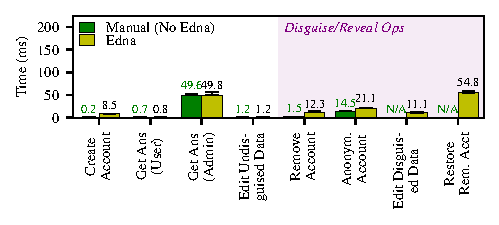
\includegraphics[width=.8\columnwidth]{figs/websubmit_op_stats}
\caption{WebSubmit (2k users, 80 answers/user).}
\label{f:ops-websubmit}
\end{subfigure}
\begin{subfigure}[b]{\columnwidth}
    \centering
    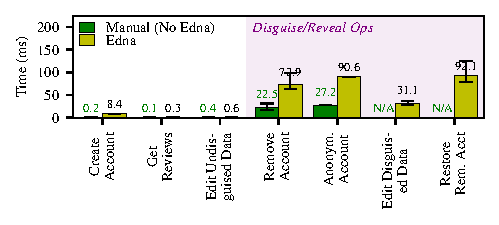
\includegraphics[width=.8\columnwidth]{figs/hotcrp_op_stats}
  \caption{HotCRP (80 reviewers, 3k total users, 200--300 records/reviewer).}
\label{f:ops-hotcrp}
\end{subfigure}
\begin{subfigure}[b]{\columnwidth}
    \centering
    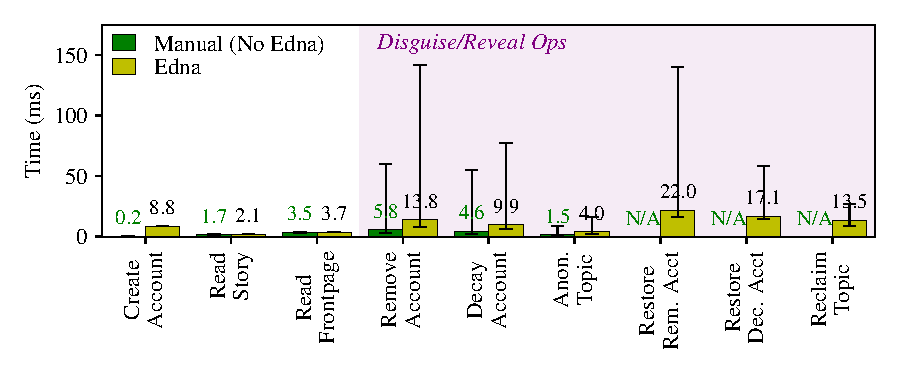
\includegraphics[width=.8\columnwidth]{figs/lobsters_op_stats}
\caption{Lobsters (16k users, Zipf-distributed data/user).}
\label{f:ops-lobsters}
\end{subfigure}
\caption{\sys adds no latency overhead to common application operations and
modestly increases the latencies of \xxing operations compared to a manual
implementation that lacks support for revealing or composition.
%
Bars show medians, error bars are 5\textsuperscript{th}/95\textsuperscript{th}
percentile latencies.}
\label{fig:client_opstats}
\end{figure}

\textbf{WebSubmit.}
%
We run WebSubmit with a database of 2k users, 20 lectures with four questions
each, and an answer for each question for each user (160k total answers).
%We implement WebSubmit account removal and answer anonymization both manually
%as an irreversible database change, and with \sys.
%
We measure end-to-end latency to perform common application operations (which
each issue multiple SQL queries), as well as \xxing and revealing operations
when possible (revealing operations are impossible in the baseline).
%
%A good result for \sys would show competitive performance with the manual
%baseline, as \sys does strictly more work (\eg encrypting \xxed
%data).
%
%Latency includes request processing in WebSubmit and \sys's
%operations, and the response to the client.
%
Figure~\ref{f:ops-websubmit} shows that common operations have comparable
latencies with and without \sys.
%
\sys adds 9ms to account creation; and \xxing
and revealing operations take longer in \sys (13.1--53.2ms), but allow users to
reveal their data and take less developer effort.
%

\textbf{HotCRP.}
%
We measure server-side HotCRP operation latencies for PC members on a database seeded with 3,080
total users (80 PC members)
%and per-user data such as paper watches;
and 550 papers with eight reviews, three comments, and four conflicts each
(distributed evenly among the PC).
%
HotCRP supports the same \xxing transformations as WebSubmit, but PC users have more
data (200--300 records each), and HotCRP's \xxing transformations mix deletions and
decorrelations across 12 tables. %, so we would expect higher latencies.
%

%
Figure~\ref{f:ops-hotcrp} shows higher latencies in general, even for the manual
baseline, which reflects the more complex \xxing transformations.
%
\sys takes 63.8--84.6ms to \xx and reveal a PC member's data, again owing to the
extra cryptographic operations necessary.
%
HotCRP's account anonymization is admin-applied and runs for all PC members, so
its total latency is proportional to the PC size.
%
With 80 PC members, this transformation takes 6.8s, which is acceptable for a
one-off operation.
%
As before, \sys adds small latency to common application operations, and 9ms to
account creation.
%

\textbf{Lobsters.}
%
We run Lobsters benchmarks on a database seeded with 16k users, and
120k stories and 300k comments with votes, comparable to the late-2022 size of
production Lobsters~\cite{lobsters}.
%
Content is distributed among users in a Zipf-like distribution according to
statistics from the actual Lobsters deployment~\cite{lobsters-data}, and 20\% of
each user's contributions are associated with the topic to anonymize.
%
The benchmark measures server-side latency of common operations and
\xxing/revealing transformations.
%
%Because Lobsters users have far more variable amounts of
%data, we expect higher variability in latencies.
%and we measure the account
%decay \xxing transformation (and subsequent restoration) in addition to GDPR-compliant
%account removal and restoration.
%
%Lobsters does not support editing decayed contributions.
%
%As the amount of data per user follows a Zipf-like distribution, we would
%expect \xxing some users to be more expensive than others.
%

%
The results are in Figure~\ref{f:ops-lobsters}.
%
The median latencies for entire-account removal or decay are small (9.7--13.4ms
for \sys, and 4.0--5.2ms for the baseline), since the median Lobsters user has
little data. Revealing \xxed accounts takes 13.1--17.6ms in the median.
%
Highly active users with lots of data raise the 95\textsuperscript{th} percentile
latency to 100--180ms for \xxing and 45--80ms for revealing.
%
Topic anonymization touches less data and is faster than
whole-account transformations, taking 3.6ms and 13.1ms for the median user to
\xx and reveal, respectively.
%

\textbf{Summary.}
%
\sys necessarily adds some latency compared to manual, irreversible data
removal, since it encrypts and stores \xxed data.
%
However, most \xxing transformations are fast enough to run interactively as
part of a web request.
%
Some global \xxing transformations---\eg HotCRP's conference anonymization over
many users---take several seconds, but an application can apply these
incrementally in the background, as in Lobsters account decay.
%
%We next break down these costs.
%
%%%%%%%%%%%%%%%%%%%%%%%%%%%%%%%%%%%%%%%%%%%%%%%%%%%%%%%%%%%%%%%%%%%%%%%%
\subsection{Performance of Reveals with Database Changes}
\label{s:eval:updates}

We next look at how operating in the presence of schema migrations or
conflicting application updates changes with \sys, and how it affects \sys's
reveal performance. 

First, we look at the cost of invoking \sys to record updates when the
application performs updates or schema migrations in Lobsters.
%
Applying these changes themselves equates to modifying all 120k stories (\eg URL 
normalization) and/or changing the database schema.  The URL normalization
application update takes 5.63s, the longest of all updates.
%
This matches the optimized bulk update time of 6s in the deployed Lobsters
application, which batch updates all stories with the normalized URL. The
unoptimized version that updates stories one-by-one takes 1789s.
%

%
Adding the \texttt{show\_email} attribute to the \texttt{users} table takes
82ms, and 
%
creating and populating the \texttt{story\_texts} table, and removing a column
from the \texttt{stories} table takes 4.93s.

%
Invoking \sys's hook to insert a new application update in \sys's replay log
takes on average 0.58ms, a negligible amount compared to the time to perform the
update/migration. This includes the time to persist the update (one database
insert query) and add it to \sys's in-memory update replay log.
%
%Each entry in the replay log requires \todo{XXX} bytes of memory (and disk, if
%persisted). \lyt{Not persisted? They're also function pointers, so I'm not sure
%*how* to encode them / find the size of the actual code block?}
%

%
We next evaluate the latency of reveal operations in Lobsters when the global
database changes described in \S\ref{s:casestudies:updates} have been applied
after reveal.
%
The effects of performing updates increases with the amount of disguised data a
user wants to reveal. For our support updates, the main overheads come from
revealing disguised stories, which increases by 0.5--0.8ms per disguised
story.
%
Our chosen updates either affect diff records containing \texttt{users} or
\texttt{stories} data. URL normalization and reorganizing into
\texttt{story\_texts} both affect \texttt{stories}, and take on average
0.4--0.5ms and 0.02ms respectively when applied to the original and placeholder
rows for a single \texttt{stories} diff record. 
%
The main cost of URL normalization comes from initializing a URL normalizer
object ($\approx$0.3ms).
\todo{we could amortize this by putting the normalizer in Edna or something, but
this would be cheating... or batching all story diff records into one update.}
%
Restoring a stories diff record also requires an additional query to reveal a
\texttt{story\_texts} table row, incurring a 0.1--0.3ms cost per story.
%
(Revealing other table diff records adds only the cost of checking whether to
apply the updates, which takes 0.01--0.02ms per diff record).
%
In total, we observe that users with very few (\eg $<5$ posted stories) incur
negligible additional overheads , but users with lots of data incur moderate
overheads proportional to the number of their stories (\eg $\approx$400ms to reveal
an account with 600-700 stories).
%\eg 673 stories and 1971 comments

\todo{there's extra overheads for the updates test simply because db queries take 0.1ms longer for
every table... not really sure what to do about this (could this be because the
database has been globally updated?)}

%
Adding \texttt{show\_email} to \texttt{users} adds negligible overheads
($<0.01$ms per user), as this simply appends a column to the in-memory row.
This update also does not increase the number of queries to reveal a user
record.
%

%%%%%%%%%%%%%%%%%%%%%%%%%%%%%%%%%%%%%%%%%%%%%%%%%%%%%%%%%%%%%%%%%%%%%%%%

\subsection{\sys Performance Drill-Down}
\label{s:eval-additional}
%\lyt{made this a subsubsection}

\begin{figure}[h]
    \centering
    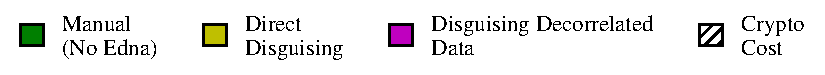
\includegraphics[width=\columnwidth]{figs/composition_legend}
    \begin{subfigure}[b]{.48\columnwidth}
        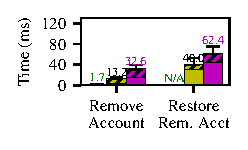
\includegraphics[width=\columnwidth]{figs/composition_stats_websubmit}
        \caption{WebSubmit}
        \label{f:comp-websubmit}
      \end{subfigure}
      \begin{subfigure}[b]{.48\columnwidth}
          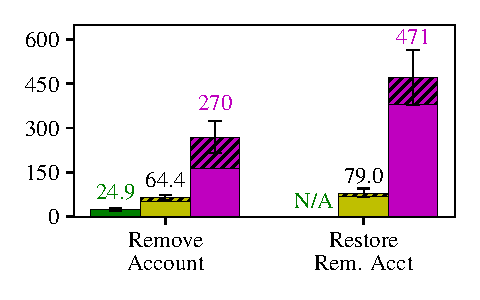
\includegraphics[width=\columnwidth]{figs/composition_stats_hotcrp}
          \caption{HotCRP}
        \label{f:comp-hotcrp}
      \end{subfigure}
    \caption{Applying \xxing transformations to previously-decorrelated accounts
      increases latency linear in the number of pseudoprincipals involved.
      %to the amount of data touched, as \sys performs
      %3--5.5$\times$ and restoration by 5.7--10$\times$ as \sys
      %cryptographic operations linear in the number of pseudoprincipals
      %involved.
      Hatched lines indicate the proportion of cost attributed to
      cryptographic operations.}
    \label{f:composition}
\end{figure}

We next break down the cost of \sys's operations into the cost of database
operations and the cost of cryptographic operations.
%
%\sys's basic API performs some computation (which we expect to be quick) as
%well as two operations that could cause bottlenecks, namely data encryption
%and decryption and access to \sys's database.
%
%\sys's high-level API additionally performs queries on the application database.
%
\lyt{Each disguise and reveal operation requires decoding of JSON specifications
into \sys-specific Rust datatypes; this takes $\approx0.1$ms on average. This
could be offloaded to registering each specification with \sys when the
application starts, allowing \sys to decode them in advance.}
%
\sys's database operations are fast; in our prototype, they generally take
$0.2$--$0.3$ms but vary depending on the amount of data touched.
%
%Database query latency depends on the amount of data
%touched, but is normally $<$1ms in our case studies.
%
\sys's cryptographic operations are comparatively expensive.
%; Figure~\ref{f:opstats} shows their cost.
%
PBKDF2 hashing for private key management incurs a 8ms cost and affects account
registration and operations on \xxed data that reconstruct a user's private key;
this accounts for up to 79\% of these operations' cost when the operation issues
only a few database queries.
%
%This appears during registration (generating password-based credentials from the
%private key), as well as operations on \xxed data that reconstruct the private key
%(\ie editing or restoring \xxed data).
%
%Applications that only wish to support private keys as reveal credentials can tell
%\sys to skip PBKDF hashing and secret sharing, eliminating this cost.
%

Encryption and decryption incur baseline costs of 0.1ms and 0.02ms respectively;
their cost grows linearly with data size.
%
In the common case, \xxing or revealing data performs two cryptographic
operations: one to encrypt/decrypt the diff and speaks-for records, and one to
encrypt/decrypt the ID at which they are stored.
%

\sys also generates a new key for each pseudoprincipal created, which takes
0.2ms.
\sys's cryptography accounts for up to 35\%
%1--35\%
of the cost of \xxing/revealing operations such as account removal or
anonymization; this proportion decreases as the number of database
modifications made by a transformation increases.
%Disguising undisguised data performs a single encryption, and
%A new disguise or reveal operation requires a single encryption/decryption
%when a single disguise to the data.
%
When the application applies multiple \xxing transformations and \xxs the
data of pseudoprincipals, doing so may require several encryptions/decryptions.
%
We evaluate this cost next.
%

%
%\lyt{ADDED THIS.}
%%
%\sys's \xxing transformations (\eg remove account) incur costs proportional to
%the amount of data a user owns: decorrelating a user's per-lecture answers in
%WebSubmit, for example, requires retrieving the user's answers,  inserting
%per-lecture pseudoprincipals, and update queries (one per each of the 80
%answers) to rewrite answers to correlate to pseudoprincipals. This results in a
%total of $\approx$18ms simply to perform database modifications.
%%
%For each of these decorrelations, \sys produces speaks-for records that are then
%encrypted and persisted, accounting for the remaining 2ms costs.
%%
%
%The cost of \sys's revealing transformations (\eg restore account) can also be
%explained as a breakdown between database query overheads and decryption
%overheads.
%%
%Restoring removed answers first requires decrypting a user's diff tokens.
%%
%For each of a user's 80 answers, \sys performs three selection queries for
%consistency checks to ensure that reinsertion can correct proceed (0.4-0.5ms)
%and inserts the answer (0.2ms).
%%
%Total restoration of a user's answers thus takes $\approx$50ms; the remaining 1-2ms cost
%comes from clearing the diff and speaks-for tokens of the revealed
%transformation, which requires both a decryption and a database deletion query.
%%
%Wrapping all reveal queries in a transaction did not meaningfully improve
%performance.
%%
%

\subsection{Composing \Xxing Transformations.}
\label{s:eval-composition}
% \lyt{this is now under \sys op performance}.

%
To understand the overhead of composing transformations in \sys,
we measure the cost of composing account removal on top of
%from an application that already invoked
a prior \xxing transformation to anonymize and decorrelate all users' data.
%
We consider WebSubmit and HotCRP, and compare three setups: \one{} manual
account removal (as before); \two{} account removal and restoration
\emph{without} a prior anonymization \xxing transformation; and \three{} account
removal and restoration \emph{with} a prior anonymization \xxing transformation.
%
With prior anonymization, a subset of the user's data has already been decorrelated
when removal occurs, and removal therefore performs per-pseudoprincipal encryptions of
\xxed data with pseudoprincipals' public keys.
%by the first \xxing transformation, and \sys
%
%This requires individually encrypting data with each pseudoprincipal's
%public key.
%
Restoring the removed, anonymized account must then individually decrypt
pseudoprincipal records and restore them.
% to both restore and then clear them.
%
Hence, \xxing and revealing in the third setup should take time proportional to
the number of pseudoprincipals created by anonymization.
%

%
Figure~\ref{f:composition} shows the resulting latencies.
%
WebSubmit account removal and restoration latencies increase by $\approx$1ms per
pseudoprincipal (18.2ms and 21.8ms respectively); 50\% of this increased cost
comes from the additional, per-pseudoprincipal encryption and decryption of
records, the rest comes from database operations.
%
HotCRP removal and restoration latencies also increase by $\approx$1ms
per pseudoprincipal (191.2ms and 230.4ms respectively); again, cryptographic
operations add $\approx$0.5ms per pseudoprincipal, and the remaining cost
increase comes from per-pseudoprincipal database queries and
updates.
%querying-for and per-pseudorpicnipal
%
WebSubmit and HotCRP do not create new references to pseudoprincipals
after data gets disguised, but if they did, \sys would need to issue additional
per-pseudoprincipal queries to rewrite or remove these references (if configured
to do so).
%
Compared to accounts in WebSubmit, accounts in HotCRP have more data and
14--15$\times$ more pseudoprincipals after anonymization, which accounts for the
larger relative slowdown.
%
%HotCRP particularly demonstrates how cryptographic operations grow comparatively
%more expensive: from 21\% of the cost to 41\% for account removal, and from 8\%
%to 25\% for account restoration.
%
%
%Restoring an account (\ie undoing a composed disguise) is more expensive than removing an
%account (\ie composing a disguise atop another) because
%decryption is more expensive than encryption (Figure~\ref{f:opstats}).
%

%
Importantly, \xxing latencies stabilize when \sys composes further \xxing
transformations: since cost is proportional to the number of pseudoprincipals
affected, latency does not grow once the application has maximally decorrelated
data (to one pseudoprincipal per record), as done by HotCRP anonymization.
%\lyt{XXX} HotCRP's anonymization
%performs maximal decorrelation, and the subsequent account removal demonstrates
%this maximal cost.
%


% %
% The experiment composed an interactive \xxing transformation (account removal) atop a
% non-interactive one (anonymization).
% %
% This benefits from the optimization for interactive \xxing transformations mentioned in
% \S\ref{s:composition}: the natural principal introduces locators for
% pseudoprincipal-owned bags that \sys forgot, which helps avoid a locator
% decryption on revealing the composed \xxing transformation.
% %
% Composing a non-interactive \xxing transformation requires this extra encryption/decryption
% as \sys store the locators; but the cost remains linear in the number of
% pseudoprincipals touched.
% %

\section{\sys Overheads}
\label{s:eval-overheads}

\sys adds both space and compute overheads to the application; we measure the
impact of these next.

\subsection{Space Used By \sys.}

%\begin{figure*}[t]
%\centering
%\begin{tabular}{ccc}
%    & \textbf{Pre-Delete (MB)} & \textbf{Post-Delete (MB)} \\
%\hline
%    App DB (does not include metadata) & 261 & 290\\
%    Encrypted Bags (Mem) & 0 & 34.3\\
%    Encrypted Locators (Mem) & 0 & 1.9\\
%    Principal Metadata (Mem) & 1.8 & 16.5\\
%    Shares Metadata (Mem) & 2.0 & 2.0\\
%    Encrypted Bags (Disk) & 0 & 35.1\\
%    Encrypted Locators (Disk) & 0 & 0.4\\
%    Principal Metadata (Disk) & 2.6 & 14.1 \\
%    Shares Metadata (Disk) & 8.9 & 8.9\\
%\end{tabular}
%    \caption{Amount of data before and after 10\% of users remove their accounts. Edna adds an extra
%    110MB on disk (and 44MB in memory).}
%  \label{f:storage}
%\end{figure*}
%
To understand \sys's space footprint, we measure the size of all data stored
on disk by \sys before and after 10\% of users in Lobsters (1.6k users)
remove their accounts.
%
%
Cryptographic material adds overhead and each generated pseudoprincipal adds an
additional user to the application database; \sys also stores data for each
registered principal (a public key and a list of opaque indexes) as well as
encrypted records.
%
%Clients keep track of their credentials, but these are small and encoded
%in application-specific ways.


%
\sys's record storage uses 12 MB, which grows to
58.5 MB after the users remove their accounts, and the application database
size increases from 261 MB to 290 MB (+11\%).
%
(\sys also caches some of this data in memory.)
%
The space used is primarily proportional to the number of pseudoprincipals
produced: each pseudoprincipal requires storing an application database record, a
speaks-for record, and row in the principal table.
%
In this experiment, Lobsters produces 78.1k pseudoprincipals.
%
%Storing a private key is necessary if the application wants to further
%disguise decorrelated data, but avoidable if disguises cannot compose.
%
%In addition, each pseudoprincipal inserts a public key into \sys's
%metadata, adding $\approx$0.3 KB per pseudoprincipal and 24 MB combined,
%
%
\sys removes the public keys and database data for the 1.6k removed principals, but
stores encrypted diff records with their information, which uses another 2.2 MB.
%
%These diff records amount to a small overhead (2.2MB).
%
%2.2MB is 0.8\% of the original Lobsters database size of 261 MB.

%%%%%%%%%%%%%%%%%%%%%%%%%%%%%%%%%%%%%%%%%%%%%%%%%%%%%%%%%%%%%%%%%%%%%%%%
\subsection{Impact On Concurrent Application Use.}
\label{s:eval-conc}

%
%Web applications serve many concurrent users, most of whom are simply using the
%application.
%
%Occasionally, a user (or an admin, or a cron job) will initiate a \xxing
%transformation via \sys.
%
For \sys to be practical, the throughput and latency of normal application requests
by other users must be largely unaffected by \sys's \xxing and revealing operations.
%
%If an expensive \xxing transformation---such as a popular Lobsters user removing their
%account---blocked application processing for all other users, developers would
%be rightly leery of \sys.
%

\begin{figure}[t]
    \centering
    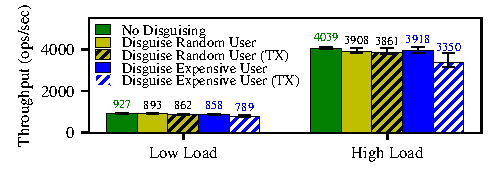
\includegraphics[width=\columnwidth]{figs/lobsters_concurrent_results}
    \caption{Continuous \xxing/revealing operations in Lobsters
    have a <7\% impact on application request
    throughput when disguising a random user; an extreme case of a
    heavy-hitter user with lots of data repeatedly \xxing and revealing
    causes a 3--17\% drop in throughput.}
    \label{f:concurrent-lobsters}
\end{figure}

%
We thus measure the impact of \sys's operations on other concurrent requests
in Lobsters.
%
In the experiment, a set of users make continuous requests to the
application that simulate normal use, while another distinct set of users
continuously remove and restore their accounts.
%
\sys applies \xxing transformations sequentially, so only one transformation
happens at a time.
%
% (This is realistic, as the UI can process later requests asynchronously; it also
% avoids \sys having to reason about overlapping data between two or more \xxing
% transformations.)
%
We measure the throughput of ``normal'' users' application operations, both
without \sys operations (the baseline) and with the application continuously
invoking \sys.
%
The Lobsters workload is based on request distributions in the real
Lobsters deployment~\cite{lobsters-data}.
% users read stories, load the frontpage,
% vote and comment, and post stories.
%

%
Since users' \xxing/revealing costs vary in Lobsters, we measure the
impact of \one{} randomly chosen users invoking account removal/restoration, and
\two{} the user with the most data continuously removing and restoring their
account (a worst-case scenario).
% , since this overlaps most with the data touched by normal users).
%
We show throughput in a low load scenario ($\approx$20\% CPU load),
and a high load scenario ($\approx$95\% CPU load).
%
Finally, we measure settings with and without a transaction for \sys
transformations.
%
%The latter makes sense if the application wishes to avoid exposing
%partially-\xxed data to other clients.
%
A good result for \sys would show little impact on normal operation throughput
when concurrent \xxing transformations occur.
%

%
Figure~\ref{f:concurrent-lobsters} shows the results.
%
If a random user disguises and reveals their data (the common case),
normal operations are mostly unaffected by concurrent \xxing and revealing:
throughput drops $\le$3.7\% without transactions and $\le$7.0\% with transactions.
%
Constantly \xxing and revealing the user with the most data (the worst-case
scenario) has a larger effect, with throughput reduced by up to $7.4$\%
(without transactions) and up to $17$\% (with transactions, high load).
%5.8\% in low load, 2.6 high
%13.3\% in low load, 16.3 high
%dropping by at most 4.6\%---by concurrent \xxing of a random user
%(with and without transactions) and of the most expensive user (without
%transactions); \xxing the most expensive user with transactions does, however,
%impact performance by 11.9\%.
%%
%Under high load, the relative impacts are similar: the throughput when
%concurrently \xxing a random user (with and without transactions) and the most
%expensive user (without transactions) drops by $\le 4.4$\%; and when disguising the
%%most expensive user with transactions, drops by 17.1\%.
%
%\lyt{XXX Note: drop w/out txn is actually more for low load than high load.}
%10% low load
%
%The throughput of normal application requests under low load, with account
%removals and restorations of either random users or the most expensive user,
%remains relatively unaffected at 1.3k ops/s (decreasing by $<$100 ops/s, or
%6\%).
%%
%Account removal and restoration under high load results in a slight decrease
%(1.8\%) in throughput (transactions decrease throughput by 3.8\%), but
%throughput remains high ($>5$ops/ms).
%

This shows that \sys's \xxing and revealing transformations have acceptable
impact on other users' application experience in the common case.
%and operations over \xxed data
%
%\ms{Did we lose a sentence about account removals under low load here? The following doesn't quite flow from the prior point}
%
%Account removals and restorations under low load take longer, with
%the expensive user's account removal and revealing taking 4.4 and 3.6 seconds
%respectively.
%

The latency of disguising operations depends on load:
the expensive user's account removal and revealing take 4.4 and 3.6 seconds
under high load, and 3.3 and 2.6 seconds under low load.
%
This is acceptable: 50\% of data deletions at Facebook take five minutes or
longer to complete~\cite{delf}.
%

%low load
%-0.03667745415
%-0.07011866235
%-0.07443365696
%-0.1488673139

%high load
%-0.03243377074
%-0.04431790047
%-0.02995791037
%-0.1705867789
%cheap disguise 17 27 39
%cheap restore 118 291 472
%cheap disguise txn 22 35 49
%cheap restore txn 118 288 467
%expensive disguise 3212 3517 3693
%expensive restore 2693 2811 2979
%exp txn delete 3029 3269 3481
%exp txn restore 2422 2612 2868
%expensive disguise 4105 4373 4594
%expensive restore 3704 3903 4317
%exp txn delete 4135 4400 4592
%exp txn restore 3542 3661 3785

%%%%%%%%%%%%%%%%%%%%%%%%%%%%%%%%%%%%%%%%%%%%%%%%%%%%%%%%%%%%%%%%%%%%%%%%
\subsection{Comparison to Qapla}
\label{s:eval-qapla}

We compare \sys's performance and the effort to use \sys to an implementation of
the same disguising and revealing functionality for WebSubmit in Qapla.
%

%
\textbf{Effort.}
%
Specifying \xxing transformations as Qapla policies requires far more
explicit reasoning about transformations' implementations and their
compositions.
%
In Qapla, a developer would realize \xxing transformations via metadata flags
that they add to the schema (\eg \fn{is\_deleted} for removed data) and toggles in
application code. They then provision Qapla with a predicate that checks if
this metadata flag is \fn{true} before returning a row.
%
Developers must carefully craft Qapla's predicates, which grow in complexity
with the number of \xxing transformations that can compose. For example, an
application supporting both account removal and account anonymization must
combine predicates such that removal always takes precedence. Each additional
transformation increases the number of predicates whose combinations the
developer must reason about.
%
Developers must also optimize Qapla predicates (\eg reducing joins, adding
schema indexes and index hints) to achieve reasonable performance.

%
To modify data, the application developer can use Qapla's ``cell blinding''
mode, which dynamically changes column values (to fixed values) based on a
predicate before returning query results.
%
The developer must manually implement more complex modifications and
decorrelation (\ie creating pseudoprincipals and rewriting foreign keys).
%

%
Realizing WebSubmit transformations in Qapla required 576 lines of C/C++, and
110 lines of Rust to add pseudoprincipal, modification, and decorrelation
support.
%(as well as the required 300 lines of Rust code to add
%HTTP endpoints).
%

Overall, Qapla requires more developer effort than \sys, particularly in writing
composable and performant predicates, and manually implementing modifications
and decorrelations. However, Qapla's approach does make some things easier.
%
Because data remains in the database, revealing simply requires toggling
metadata flags, and data to reveal can adapt to database changes (\eg
schema updates). But keeping the data in the database also means that developers cannot use Qapla to
achieve GDPR-compliant data removal. %, as the data remains in the database.

%
\begin{figure}[t]
  \centering
      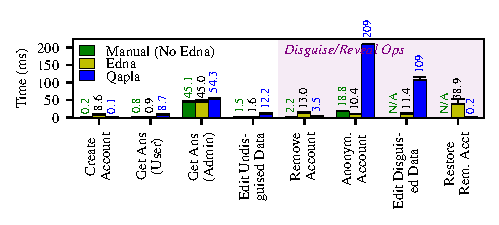
\includegraphics[width=\columnwidth]{figs/websubmit_qapla_op_stats}
    \caption{\sys achieves competitive performance with a manual baseline and
    outperforms Qapla on nearly all common WebSubmit operations (2k users,
    80 answers/user).
    Bars show medians, error bars are 5\textsuperscript{th}/95\textsuperscript{th}
    percentile latencies.}
  \label{f:qapla_ws_opstats}
\end{figure}

%
\textbf{Performance.}
% comparable with \sys.
%
We measure Qapla's performance (Figure~\ref{f:qapla_ws_opstats}) on the same
WebSubmit operations (Figure~\ref{f:ops-websubmit}).
%
Qapla performs well on operations that require only writes, since Qapla does not
rewrite write queries.  Removing and restoring accounts requires only a single
metadata flag update in Qapla, whereas \sys encrypts/decrypts user data and
actually deletes it from the database.
%
However, Qapla rewrites all read queries, so Qapla performs poorly on operations
that require reads, such as listing answers and editing (disguised or
undisguised) data.
%
Qapla's query rewriting takes $\approx$1ms, and rewrites \fn{SELECT} queries in
ways that affect performance (\eg adding joins to evaluate predicates).
%
Overall, \sys achieves better performance on common operations.

%
%Furthermore, \sys achieves better performance than Qapla on common operations.


%%%%%%%%%%%%%%%%%%%%%%%%%%%%%
\section{\syscrypt}
\label{s:eval-cryptdb}

We combine \sys with CryptDB to evaluate the cost of composing \sys's guarantees
with those of encrypted databases.
%
%To harden \sys's security guarantees, developers can deploy an \sys-enabled
%application atop an encrypted database such as CryptDB~\cite{cryptdb}.
%
CryptDB protects un\xxed database contents against attackers who compromise
the database server itself (with some limitations~\cite{grubbs}), in addition
to \sys-like protections for \xxed data.
%
%We refer to the combination of \sys and CryptDB as \syscrypt.
%

%
%\textbf{Proxy Encryption and Decryption.}
\syscrypt operates in CryptDB's threat model 2 (database server and proxy can be
compromised).
%
A developer using \syscrypt deploys the application (and \sys) atop a proxy that
encrypts and decrypts database rows.
%
%\syscrypt operates on un\xxed data in the same way as CryptDB, and
%
% \syscrypt encrypts database rows with per-object keys; object keys are
% themselves
% encrypted with the public keys of the users who can access the object.
% %
% Only users who are actively using the application have their private keys in the
% proxy, so a proxy compromise only exposes the data these users have access to.
% %
% %
% On inserts or updates, \syscrypt generates keys for the new data, and encrypts
% the keys with the public key of users who own the data.
% %
% %Keys that are no longer needed are deleted from \fn{access\_keys}.
% %
% On reads, \syscrypt uses stored key-metadata to check if any accessible object key
% is associated with a retrieved object; if so, \sys decrypts the data with the
% key.
% %
% Like CryptDB, \syscrypt supports shared data by storing an encrypted copy of an
% object's key for each user who has access to the object.
%
%%
%The proxy stores encrypted object keys in an \fn{access\_keys} table mapping
%from user public key to their set of encrypted object keys.
%%
%The set of encrypted object keys is indexed by (both plaintext and encrypted)
%object identifiers, which allows for efficient lookup of object keys to encrypt
%or decrypt queries or query results.
%%
%
%\textbf{Developer Experience.}
%To use \syscrypt, application developers specify which users can
%access what data (\eg by specifying foreign keys that indicate ownership of
%objects).
%
%Developer-provided \xx specifications have this additional role in
%\syscrypt. \hmng{ this feels unclear. How do they do this? Just in the sense that it's
%implicitly already given in the schema description that Edna gets? }
%
Queries from \sys and the application operate unchanged atop the proxy, but to
ensure proper access to user data, the application and \sys must handle user
sessions.
%
\syscrypt exposes an API to log users in and out using their credentials.  Prior to applying
transformations to a user's data, \sys performs a login to ensure that \sys has
legitimate access to their data (\eg the user, an admin, or someone sharing the
data is logged in).

%
%Because the database is encrypted, \xxing transformations
%can only operate on data that logged-in users can access.

% and provide the proxy their private keys.
%with a couple of extra requirements to provide the proxy with private keys of
%logged-in users.
%
%
%Because the database is encrypted, \xxing transformations
%can only operate on data that logged-in users can access.
%
%\sys must also add an initial login before \xxing a user's data to ensure that
%\sys has legitimate access to their data (\eg the user, an admin, or someone
%sharing the data is logged in).
%
%, similar to how the application invokes \syscrypt with the user's private key
%to reveal data.
%

\syscrypt handles keys in the same way as CryptDB: \syscrypt encrypts database rows
with per-object keys, and object keys are themselves encrypted with the public keys
of the users who can access the object.
%
After a user logs in, the application gives the proxy their private key, thus
allowing decryption of their accessible objects.
%to the proxy, and can access only those
%objects encrypted with their public keys.
%\syscrypt handles keys in the same way as CryptDB, \ie encrypting objects with
%per-object keys, and granting users access via which object keys they own.
%
% A \fn{LOGIN} request includes the user's credentials, which \syscrypt uses to
% derive the user's private key and forward it to the proxy. The proxy uses the
% private key to decrypt the user's accessible object keys and access the
% plaintext object data.
% %
% %
% A \fn{LOGOUT} request tells the proxy to remove all decrypted object keys for
% the user (and thus renders the proxy unable to decrypt the user's data).
% %
% As long as objects for a user only get created while the user is logged in,
% \syscrypt can batch-encrypt the entire set of object keys for the user when
% they log out.
% %
% Creating objects for logged-out users is possible as long as the principal's
% public key is available, but comes at a performance cost: these objects require
% creating a separately-encrypted set of object keys, which will increase
% decryption cost on the user's next login.
%

%As an optimization, if \syscrypt generates a user's object keys only when the
%user is logged in, then \syscrypt has access to the entire set of the user's
%object keys in plaintext. This lets \syscrypt batch encrypt the entire set at
%once when the user logs out.
%%
%Otherwise, if \syscrypt must store encrypted object keys for a user while the
%user is logged out, then \syscrypt does not have access to the user's
%entire set of object keys. \syscrypt must encrypt each object key individually
%with the user's public key, and store a set of encrypted keys (instead of an
%encrypted set of keys).
%%
%Regardless of how keys are encrypted, \syscrypt defers key deletion from
%\fn{access\_keys} until the user logs out.
%\lyt{Too much detail?}

%
%\syscrypt internally uses this API to ensure that \xxing transformations that
%change user ownership (perform decorrelations) properly encrypt data for
%pseudoprincipals.
%

%
%\textbf{\Xxing and Revealing.}
%

%\syscrypt requires developers to ensure that their \xx specifications touch
%only data accessible to the user who invokes the \xxing transformation.
%
%In addition, if a user's records during \xxing or revealing include speaks-for
%records, \syscrypt logs in the pseudoprincipals with the private keys encoded in
%the speaks-for records.
%
%
%\syscrypt performs data removal and data modification identically to \sys, aside
%from the initial login of users. Decorrelation additionally ensures that
%encrypted decorrelated data can still be accessed by the original user.
%
%Decorrelation, however, requires slightly more nuance: for each new
%pseudoprincipal $p$ produced, \sys must ensure that a client speaking for $p$
%can access both $p$'s account object (\eg a \fn{users} table row) and
%the objects correlated to $p$. To do so, \sys encrypts (with $p$'s key) the
%keys associated with $p$'s account and any correlated objects.
%stores an
%encrypted copy of both the pseudoprincipal object's key and an encrypted copy of
%the recorrelated object's key, so that the pseudoprincipal can access both its
%account data and its now-owned object.
%
%\ms{I don't quite understand the last bit; let's discuss.} \hmng{ seconded. }
%

%\lyt{Could just get rid of this so we're not storing so many extra keys.}
%\syscrypt allows the decorrelated, original principal owning the object to
%store encrypted copies of the pseudoprincipal object's key and retain an
%encrypted copy of the recorrelated object's key. This leaks no additional
%information about which objects the original principal was correlated with,
%while allowing the original principal to access the object if logged in after
%decorrelation (\eg to edit after anonymization).

%\textbf{Limitations.}
%
%\syscrypt's key management imposes some limitations on applications that are
%absent in plain \sys.
%
%In particular, all
%

%\textbf{WebSubmit Evaluation.}
%We run WebSubmit on top of \syscrypt so that all WebSubmit answers and user
%accounts are always encrypted in the application database.  We also support
%account removal and answer anonymization using \syscrypt.
%%
%This required modifying WebSubmit to add API calls to \syscrypt to \fn{LOGIN}
%and \fn{LOGOUT} users when they signed in and out of their user accounts.
%%
%In addition, the developer specifies which users share what data. In the case of
%WebSubmit, the admin shares answers and user accounts with all existing users;
%all other users simply own their accounts and the answers they submit.
%%
%
%%
%Because users are always logged in when they add, edit, or read their data,
%\syscrypt can optimize encryption of user object keys in \fn{access\_keys}, and
%batch-encrypts each non-admin user's set of object keys. The admin's object keys
%are individually encrypted with the admin's public key, as the admin is not
%always logged in when user answers are submitted, or accounts created.
%%

%\textbf{Takeaways.}
%While \syscrypt provides stronger guarantees, it comes with both significant
%performance cost and the additional burden on the developer to properly manage
%user login and logout (although \syscrypt can support automatic, time-based
%logouts). In addition, \syscrypt's overheads will likely only grow for more
%complex applications, for which more complex encryption and key management
%schemes must be implemented (\eg to support joins over the data of multiple
%users). However, \syscrypt demonstrates that adding the guarantees of an
%encrypted database is not fundamentally at odds with \sys, and is in fact an
%orthogonal challenge.

%
%\textbf{Implementation.}
%
The prototype supports only the CryptDB deterministic encryption scheme
(AES-CMC encryption), which limits it to equality comparison predicates. It also does not
support joins, a limitation shared with multi-principal CryptDB.
%
%Our implementation uses per-object keys that differ across tables, so
%it does not support \fn{JOIN}s, a limitation shared with multi-principal
%CryptDB (threat model 2).
%
%encrypts only sensitive object columns (\eg answer text and authors), leaving
%non-sensitive tables and columns, such as lectures, in plaintext.
%

\begin{figure}[t]
  \centering
      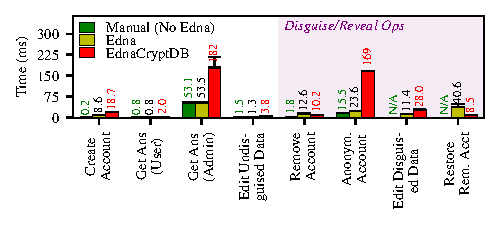
\includegraphics[width=\columnwidth]{figs/websubmit_cryptdb_op_stats}
    \caption[Latencies of Websubmit operations when implemented with
    \syscrypt.]{Latencies of WebSubmit (2k users, 80 answers/user) operations when
    implemented with \syscrypt (adding encrypted database support).
    Bars show median latency; error bars are
    5\textsuperscript{th}/95\textsuperscript{th} percentile latencies.}
  \label{f:cryptdb_ws_opstats}
\end{figure}

%
\textbf{Performance.}
We measure the latency of WebSubmit operations like before, and compare a manual
baseline, \sys, and \syscrypt.
%
\syscrypt is necessarily more expensive than \sys, and a good result for
\syscrypt would therefore show moderate overheads over \sys, and acceptable
absolute latencies.
%

%
Figure~\ref{f:cryptdb_ws_opstats} shows the results.
%
Normal application operations are 2--3$\times$ slower with \syscrypt than in
\sys, with the largest overheads on operations that access many rows, such as
the admin viewing all answers.
%
\Xxing and revealing operations are also 2--6$\times$ slower than \sys.
%

%
These overheads result from the cryptographic operations and additional
indirection in \syscrypt.
%
\syscrypt relies on a MySQL proxy, which adds latency: a no-op
version of this proxy makes operations 1.03-1.5$\times$ slower.
%proportional to the number of queries the operation issues.
%
%Further overheads come from object key management and computation necessary
%to properly encrypt query values or decrypt returned rows.
%
Cryptographic operations themselves are cheap ($<0.2$ms), but every object
inserted, updated, or read also requires lookups to find out which keys
to use, query rewriting to fetch the right encrypted rows, and
execution of more complex queries.
%

%
This is particularly expensive
when the user owns many keys (\eg the WebSubmit admin).
%
%\syscrypt maintains indexes that map object identifiers to keys for each
%user, but these indexes may not always determine which single key should be used.
%
%For example, a \fn{SELECT} query of the form \fn{SELECT * FROM answers WHERE
%email = 'some@email'} requires translating the value \fn{'some@email'}
%to ciphertexts that match all rows that encrypt answers with this email address.
%
%These rows use different keys, so after resolving the keys to use, \syscrypt
%issues a query of the form \fn{SELECT * FROM answers WHERE email IN
%(encrypted\_email1, encrypted\_email2, $\dots$)}.
%
%The index lookups to determine which keys to use and the increased query
%complexity add overhead, particularly when the user owns many keys (as in the
%case of the WebSubmit admin).
%
Admin-applied anonymization incurs the highest overhead (+143.6ms) as it issues
many queries to read user data and execute decorrelations.
%
Among the common operations,
an admin getting all the answers for a lecture
suffers similar overheads (+132.9ms).
%
%the admin possesses keys for all users's answers.
%Although \syscrypt indexes \fn{access\_keys} by object identifiers, queries that
%filter answers by partial object identifiers (\eg only lecture ID) will match
%against all keys of all users' answers, and thus require more encryptions to
%correctly apply queries.
%
%In contrast, individual users only have keys for their
%own answers, and thus often only perform one encryption (or decryption) per
%query (incurring a 2-5$\times$ overhead).

%%
%While non-trivial, these overheads may still be acceptable for practical web
%applications, as absolute latencies remain in the hundreds of milliseconds.
%%
%The latency of \xx/reveal operations, which typically run asynchronously, is
%also less critical than that of normal application operations.
%%
%
%%
%Finally, \syscrypt incurs fixed costs from \fn{LOGIN} and \fn{LOGOUT}
%operations, which prepare state in the proxy.
%%
%\fn{LOGIN} of a non-admin user takes a median of 10.2ms to decrypt and index the
%user's set of object keys;
%%: \syscrypt decrypts the user's set of object keys, and indexes each key by
%%object identifiers (\eg an answer's lecture and question IDs) for efficient key
%%lookups.
%%
%\fn{LOGOUT} of a non-admin user takes a median of 0.9ms to reencrypt the user's
%keys.
%%: \syscrypt updates, serializes, and encrypts the set of keys to store.
%%removes any keys to delete from the user's set of object keys; then
%%\hmng{When would the set of keys to be removed
%%not be all of them?}
%%
%Our \syscrypt prototype eagerly decrypts all keys for a user on login, causing
%expensive logins for users with lots of data (\eg 19s for the admin); this cost
%is not fundamental and \syscrypt could lazily decrypt keys when required.
%%, which would speed up login at the cost of additional per-query overhead.
%%

%\textbf{Security of \syscrypt.}
%
%\syscrypt combines CryptDB's protection of un\xxed data currently in the
%%database, with \sys's protection of \xxed data.
%%
%As \syscrypt executes vanilla \sys over an encrypted database, \syscrypt
%provides the same guarantees as \sys regarding confidentiality of the contents of
%\xxed data.
%%
%In addition, \syscrypt protects of the confidentiality of the contents of
%\emph{un\xxed} data in the application database against compromise of the
%database server, subject to the well-known limitations of encrypted
%databases~\cite{grubbs}.
%%
%An attacker sees only encrypted data, as every query goes through \syscrypt's
%proxy, and data stored/retrieved is encrypted/decrypted by the owning users'
%keys.
%%
%Like CryptDB, \syscrypt does not protect a user $u$'s un\xxed data if
%the attacker (1) compromises a user authorized to view $u$'s data (\eg an admin);
%or (2) compromises the application or proxy while $u$ is logged in.
%

%\textbf{\syscrypt.}
Like CryptDB, \syscrypt increases the database size (4--5$\times$ for our
WebSubmit prototype).
%
\syscrypt also stores an encrypted object key and its metadata (1KB per key) for
each user with access to that object.

%%%%%%%%%%%%%%%%%%%%%%%%%%%%%%%%%%%%%%%%%%%%%%%%%%%%%%%%%%%%%%%%%%%%%%%%

\section{Support for Application Updates and Schema Migrations}
\label{s:eval-updates}
%
In addition to the updates described and implemented in
\S\ref{s:casestudies:updates}, we inspected 20 other updates/migrations in
Lobsters from the
past three years, and classified them broadly as follows: 
\begin{itemize}[nosep] 
    \item creating tables; 
    \item removing, adding, or renaming table columns; 
    \item removing or adding table indexes;
    \item setting column constraints (\eg \texttt{NOT NULL}); 
    \item modifying column content based on deterministic functions (\eg URL normalization);
    \item generating rows for new tables based on existing table rows (\eg adding \texttt{story\_texts} when restructuring \texttt{stories}); and 
    \item updating a row based on the current state of other database tables (\eg updating the \texttt{vote\_count} of comments based on the number of votes).  
\end{itemize}
%
\sys can support all but the last category of updates, unless the 
update's output is correct no matter the state of other database tables.
%
This last category represents 2 of the 20 inspected updates.
%
%As described in \S\ref{s:design:limits}, unless it is valid application behavior
%for \eg \texttt{vote\_count} to be 0 regardless of the number of votes, \sys
%will not correctly apply an update that sets the count of votes for comments.
%
We note that these types of updates occur in applications that optimize for
performance by denormalizing their database schema; we hypothesize that this
category of update would not exist with a normalized schema.
%
These particular updates also happen to be idempotent for any rows affected, and thus
could be reapplied via \eg a cron job regularly to update revealed data.
%

%
With the exception of this last category of updates, users can still reveal
their data disguised prior to these migrations, as if the migration had occurred
with their data present in the database.

%
\section{Summary}
In our evaluation, we used \sys to add seven \xxing transformations to three web
applications. We found that the effort required was reasonable, that \sys's
\xxing and revealing operations are fast enough to be practical, and that they
impose little overhead on normal application operation.
%
